For de som kjenner meg, vet dere at bedpres er en av mine hjertesaker. Nå skal jeg dele mine beste tips for hvordan DU kan bli en \textbf{\large Bedpres Hunter}.

\begin{figure}[H]
    \centering    
    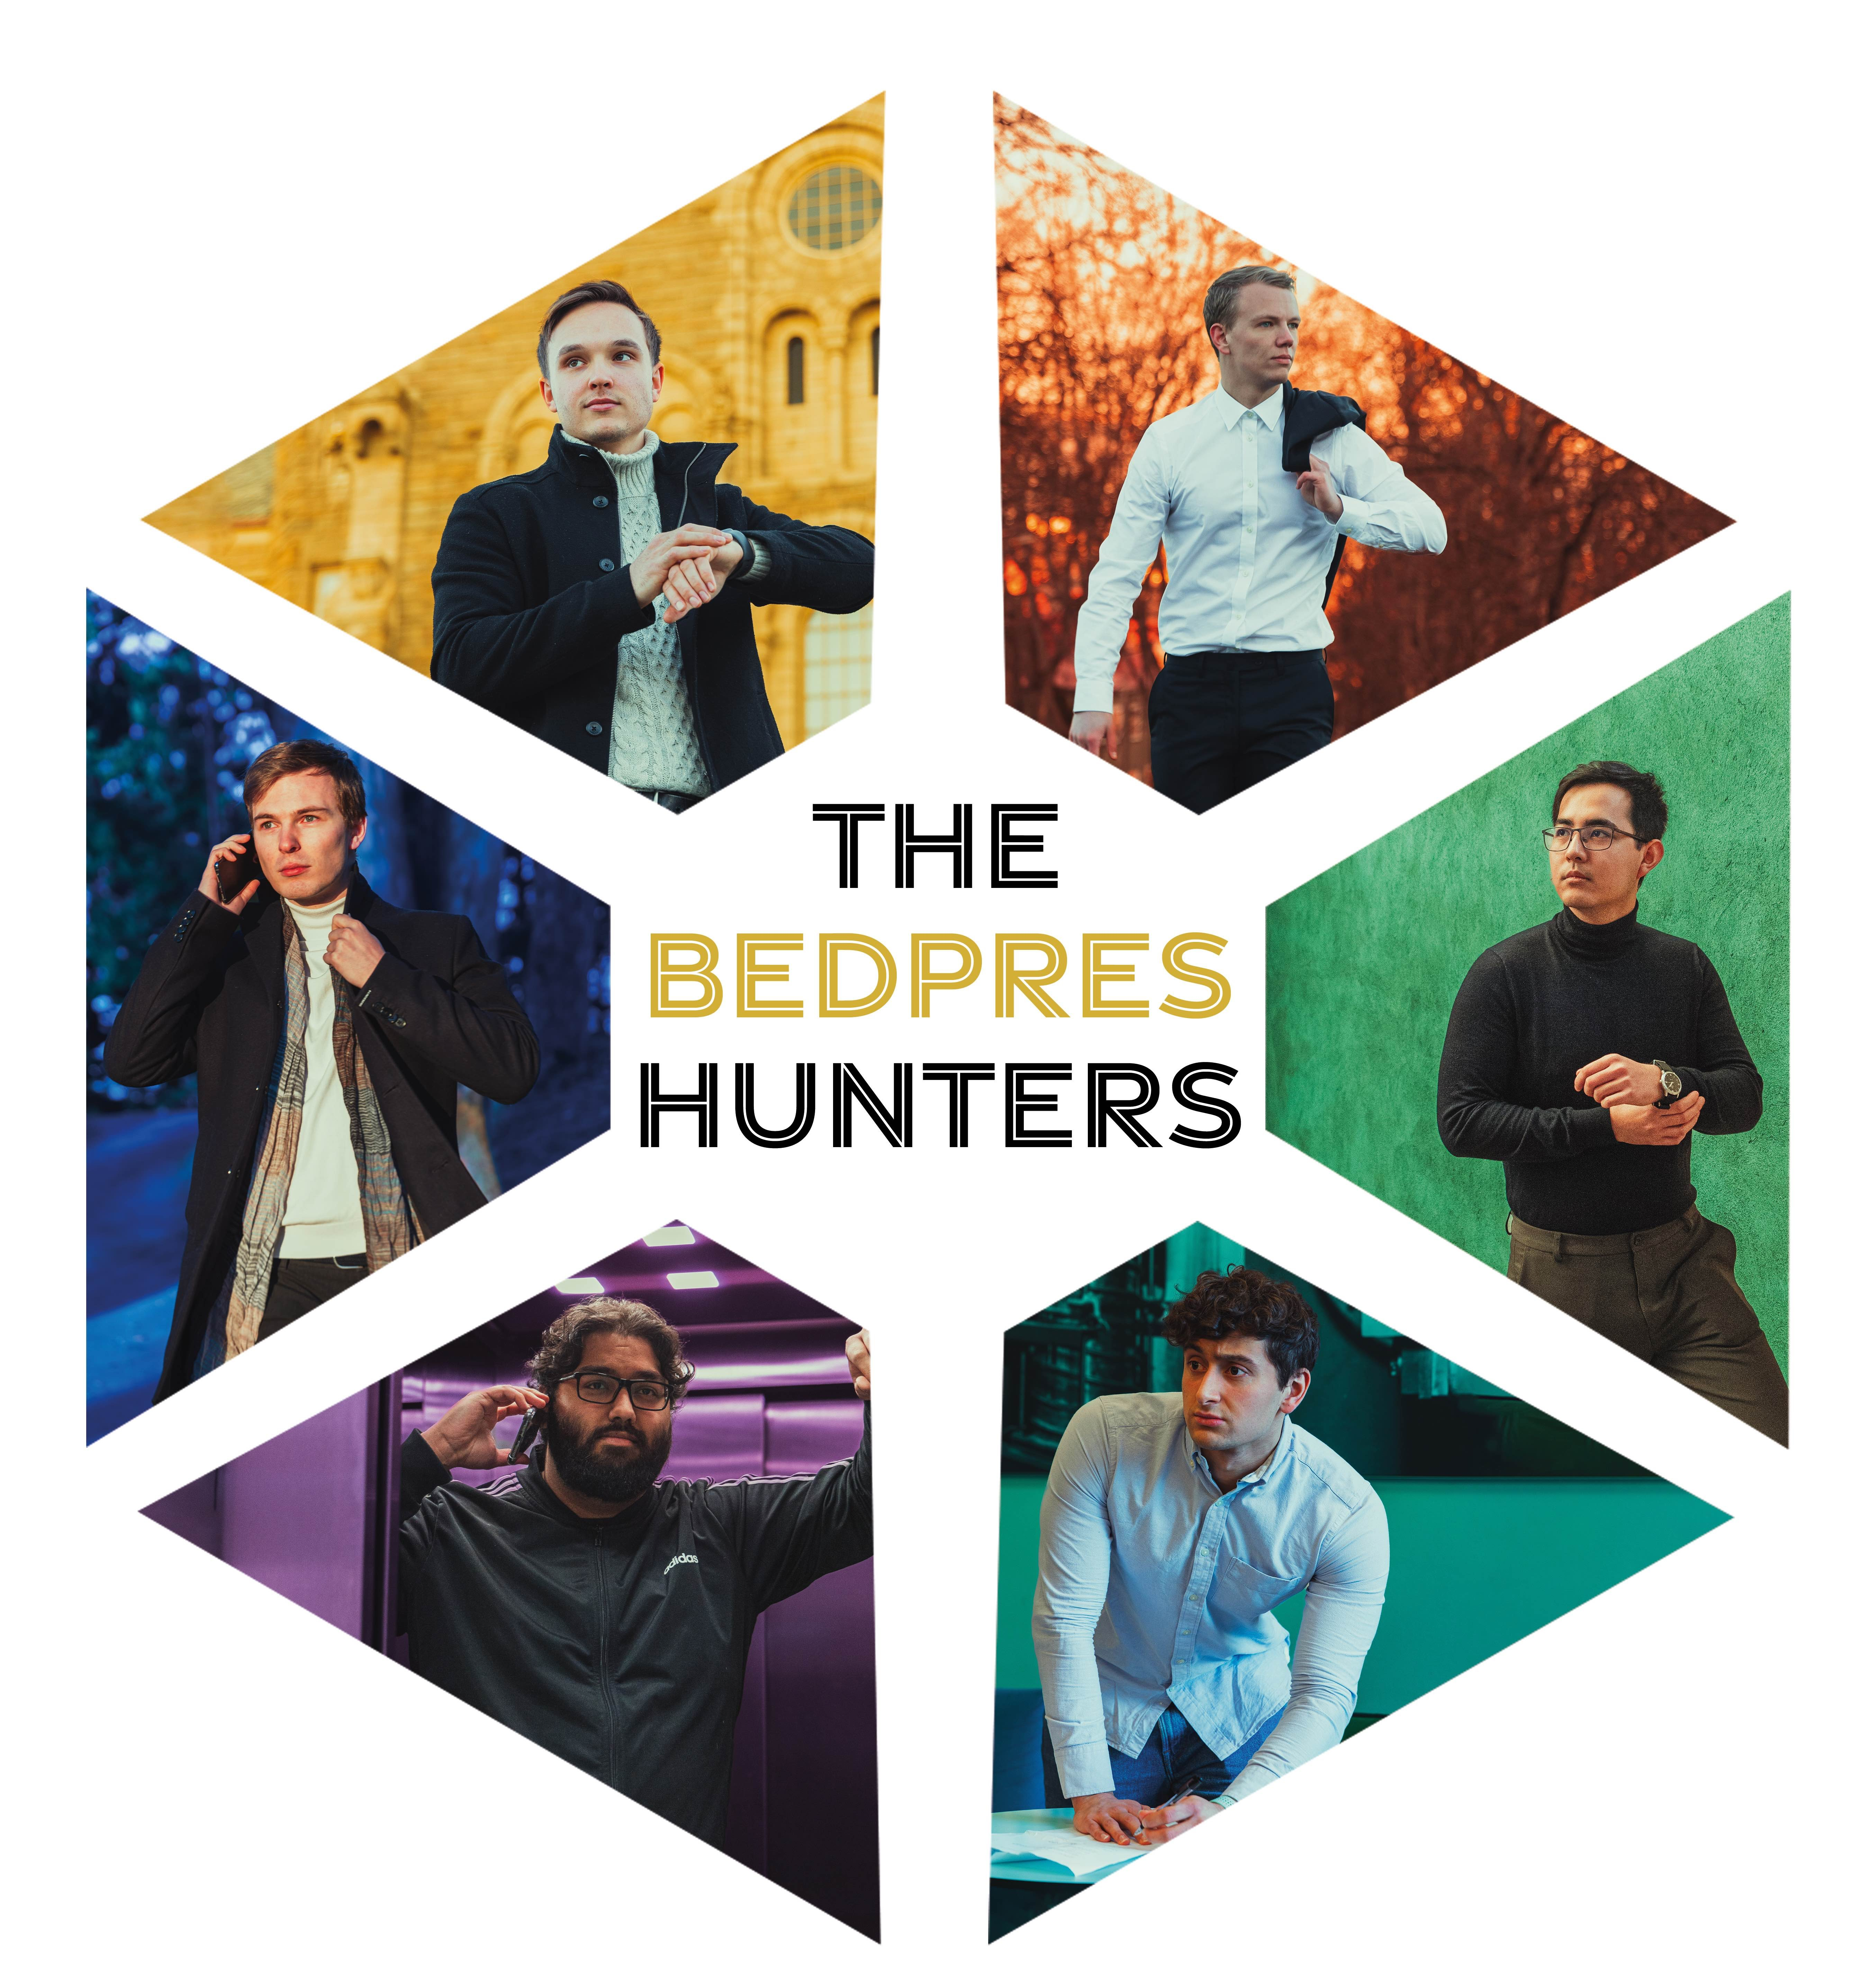
\includegraphics[width=0.7\linewidth]{images/BedpresHunters.jpg}
    \caption{Jeg brukte mange timer på plakaten, så jeg må vise den fram når jeg har muligheten ;)}
    \label{fig:bedpres}
\end{figure}




\section{Hva er bedpres?}

Hvis du aldri har hørt om ordet <<bedpres>>, så er det en forkortelse for \textit{bedriftspresentasjon}. Det er viktig at det ikke skrives som <<bedpress>>, som noen gjør. En typisk bedpres består av følgende deler:

\begin{itemize}
    \item Presentasjon av bedriften (ca. 1 time)
    \item Bespisning 
    \item Dra ut på byen (avhenger av bedrift)
\end{itemize}

Ingen bedpres er like og de vil derfor variere veldig. Noen kan tilby Pizzabakeren, mens andre kan tilby 3-retters middag med vinpakke og åpen bar på Downtown etter måltidet. 




\section{Hvorfor bedpres?}

Det er to grunner for å dra på bedpres: bli kjent med bedriften og gratis mat/drikke. Jeg drar utelukkende for det sistnevnte, men som en konsekvens så har jeg blitt kjent med ganske mange bedrifter. Nå skal jeg ramse opp en rekke bedpreser jeg har dratt på for å vise frem hva man kan forvente av slike arrangementer.

\begin{table}[H]
    \centering
    \begin{tabular}{r p{10cm}}
        \textbf{Bedrift} & PwC \\
        \textbf{Når} & Høsten 2022\\
        \textbf{Arrangør} & HC og Nabla\\
        \textbf{Oppsummering} & Ulike aktiviteter på kontoret deres i Trondheim, gruppen min vant konkurransen og fikk et handlenett med vannflaske og JBL høyttaler hver. Det var wraps og drikke under presentasjonene. Etter opplegget var det mingling og vi tømte øltappen på kontoret (ja de har øltapp på kontoret). Etter det dro vi til Solsiden og fikk spandert pizza-og pastabuffet pluss to enheter på Una Pizzeria.\\
        & \\
        \textbf{Bedrift} & Boston Consulting Group (BCG)\\
        \textbf{Når} & Høsten 2023\\
        \textbf{Arrangør} & Bindeleddet\\
        \textbf{Oppsummering} & 3-retters middag med vinpakke på Jossa (en del av Credo) og åpen bar. Undervies var det en del presentasjoner og artig underholdning. Etter middagen gikk bussen videre til Downtown (DT-torsdag altså) og der var halve 2.etasje reservert med åpen bar.\\
        & \\
        \textbf{Bedrift} &  BearingPoint\\
        \textbf{Når} & Høsten 2022\\
        \textbf{Arrangør} & Bindeleddet\\
        \textbf{Oppsummering} & Presentasjonen foregikk på Kjelhuset, før det etterpå endte på Søstrene Karlsen for en 3-retters middag. Det var åpen bar, men ikke godt egnet på en mandag ;)\\
        & \\
        \textbf{Bedrift} & Nammo Raufoss \\
        \textbf{Når} & Våren 2024\\
        \textbf{Arrangør} & Teknologiporten\\
        \textbf{Oppsummering} & Presentasjon i S8 på Stripa. Grunnet omstendighetene ble vi møtt av demonstranter som oppfordret til å boikotte bedpresen. For å unngå prikk så dro de fleste likevel og etter presentasjonen endte vi opp på Graffi Solsiden med burgermiddag og to enheter.\\
    \end{tabular}
    \caption{Oversikt over noen bedpreser.}
    %\label{tab:Casekonkurranser}
\end{table}




\section{Hvordan bedpres?}

Det finnes mange måter å komme seg inn på bedpreser. Jeg holder meg til tre kanaler:
\begin{enumerate}
    \item HC Industrikomiteen
    \item Teknologiporten
    \item Bindeleddet
\end{enumerate}

HCs \textbf{Industrikomite} har ansvar for å arrangere bedpres for medlemmer av linjeforeningen. Bedpresene er derfor alltid relevante for deltakerne, siden bedrifter spesifikt signerer avtaler med HC.

Deretter har vi \textbf{Teknologiporten} (TP), et samarbeid mellom flere studier ved Fakultet for Ingeniørvitenskap (IV – vi er NV). Her arrangeres det flere bedpreser i uken, mens HC kanskje har én i måneden. Som medlem av HC er man ikke blant de "utvalgte" ved TPs arrangementer, så det er viktig å sende en mail til den ansvarlige og spørre om MTKJ kan bli invitert. HC får penger fra TP for deltakelse på arrangementer, så jeg oppfordrer gjerne folk til å dra.

Man kan spørre hvorfor HC ikke er en del av TP, og jeg mistenker det handler om historie og misforståelser rundt kjemi. HC var ikke med da ønsket om å grunnlegge TP ble fremmet, og derfor kan de gatekeepe, fordi det ligger økonomiske interesser bak. En annen grunn er at mange misforstår hva vi egentlig studerer – vi blir ikke kjemikere, men kjemiingeniører. Som jeg nevnte tidligere da jeg snakket om spesialiseringene våre og hvordan vi ligner på andre studier, er ikke TP klar over dette og de ser derfor på oss som likestilte med \textit{Volvox og Alkymisten} (linjeforeningen for biologi- og kjemistudenter). Til tross for utfordringene, kommer man langt med en hyggelig mail, noe jeg har gjort for å få med MTKJ på flere bedpreser.

Den siste kanalen er det beryktede \textbf{Bindeleddet}, som drives av indøk-studenter. De markedsfører seg som bindeleddet mellom bedrifter og studenter ved NTNU, men de sitter igjen med all inntekten (som kan være i millionklassen). Som en konsekvens blir ofte MTKJ og andre studenter invitert til deres arrangementer. Bindeleddet sine bedpreser er de mest ekstreme, med åpen bar, 3-retters middager, og gjesteopptredener fra kjendiser. Det er også lettest å delta på bedpres via Bindeleddet, som ofte har tre bedpreser i uken. Etterspørselen etter å holde bedpres hos Bindeleddet er så høy at plassene for neste semester <<selges ut>> i løpet av timer etter at de har åpnet (angivelig).